\cleardoublepage
\begin{appendices}

\chapter{Prototipos de interfaz de usuario}
\label{anexo:prototipos_interfaz_usuario}

En este anexo se recopilan los prototipos de interfaz de usuario \textit{(mockups)} correspondientes a las principales pantallas del sistema, organizados por flujos funcionales de navegación. 

Para facilitar su interpretación visual y distinguir los roles de usuario en las capturas, se ha empleado la siguiente codificación de colores en el borde de las interfaces:

\begin{itemize}
    \item \textbf{Borde magenta:} Identifica las pantallas pertenecientes a la vista del perfil docente (profesor).
    \item \textbf{Borde cian:} Identifica las pantallas pertenecientes a la vista del perfil estudiante (alumno).
\end{itemize}

A continuación, se presentan las distintas pantallas agrupadas según la secuencia lógica de cada flujo.

\section*{Flujo de registro y autenticación}
\label{anexo:flujo_registro_autenticacion}

Engloba las pantallas destinadas a la gestión de acceso de los profesores a la plataforma. Comprende el proceso de alta de nuevos usuarios, la verificación de credenciales a través del correo institucional con código de confirmación y el formulario de inicio de sesión estándar.

\begin{figure}[H]
    \centering
    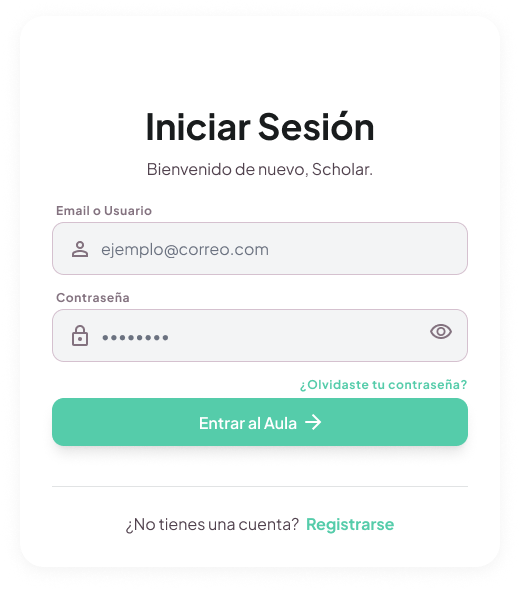
\includegraphics[width=0.45\textwidth]{mockups/01_01_iniciar_sesion.png}
    \caption[Prototipo de inicio de sesión.]{Iniciar sesión.}
    \label{fig:mockup_iniciar_sesion}
\end{figure}

\begin{figure}[H]
    \centering
    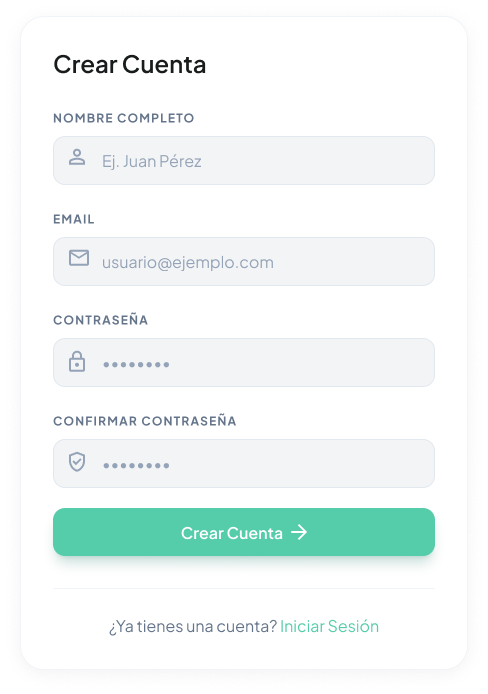
\includegraphics[width=0.5\textwidth]{mockups/01_02_crear_cuenta.png}
    \caption[Prototipo de creación de cuenta.]{Crear cuenta.}
    \label{fig:mockup_crear_cuenta}
\end{figure}

\begin{figure}[H]
    \centering
    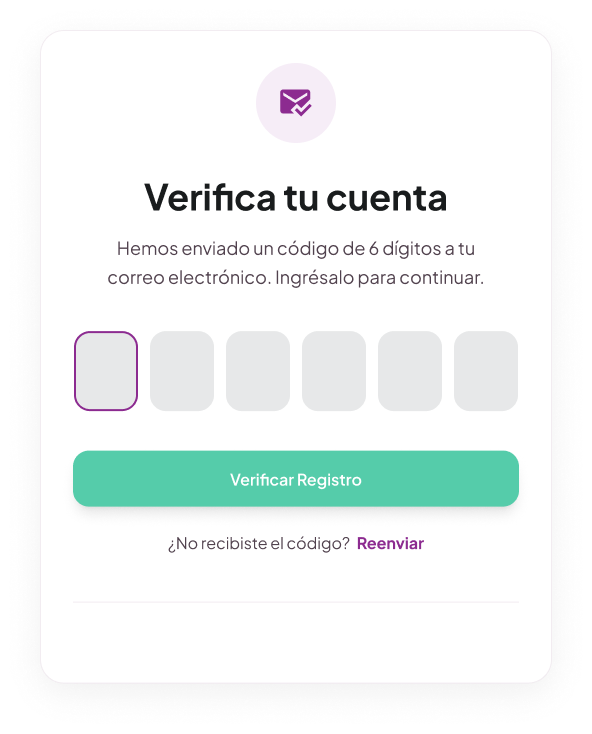
\includegraphics[width=0.53\textwidth]{mockups/01_03_verificar_cuenta.png}
    \caption[Prototipo de verificación de cuenta.]{Verificar cuenta.}
    \label{fig:mockup_verificar_cuenta}
\end{figure}

\section*{Flujo de creación de cuestionarios y gestión de salas}
\label{anexo:flujo_creacion_cuestionarios_gestion_salas}

Comprende el conjunto de interfaces utilizadas por profesor para la preparación de las clases. Incluye creación de cuestionarios (preguntas, opciones y tiempos límite), la consulta del catálogo de cuestionarios creados, la pantalla de configuración de parámetros de la sala y el estado inicial de la sala (en espera).

\begin{figure}[H]
    \centering
    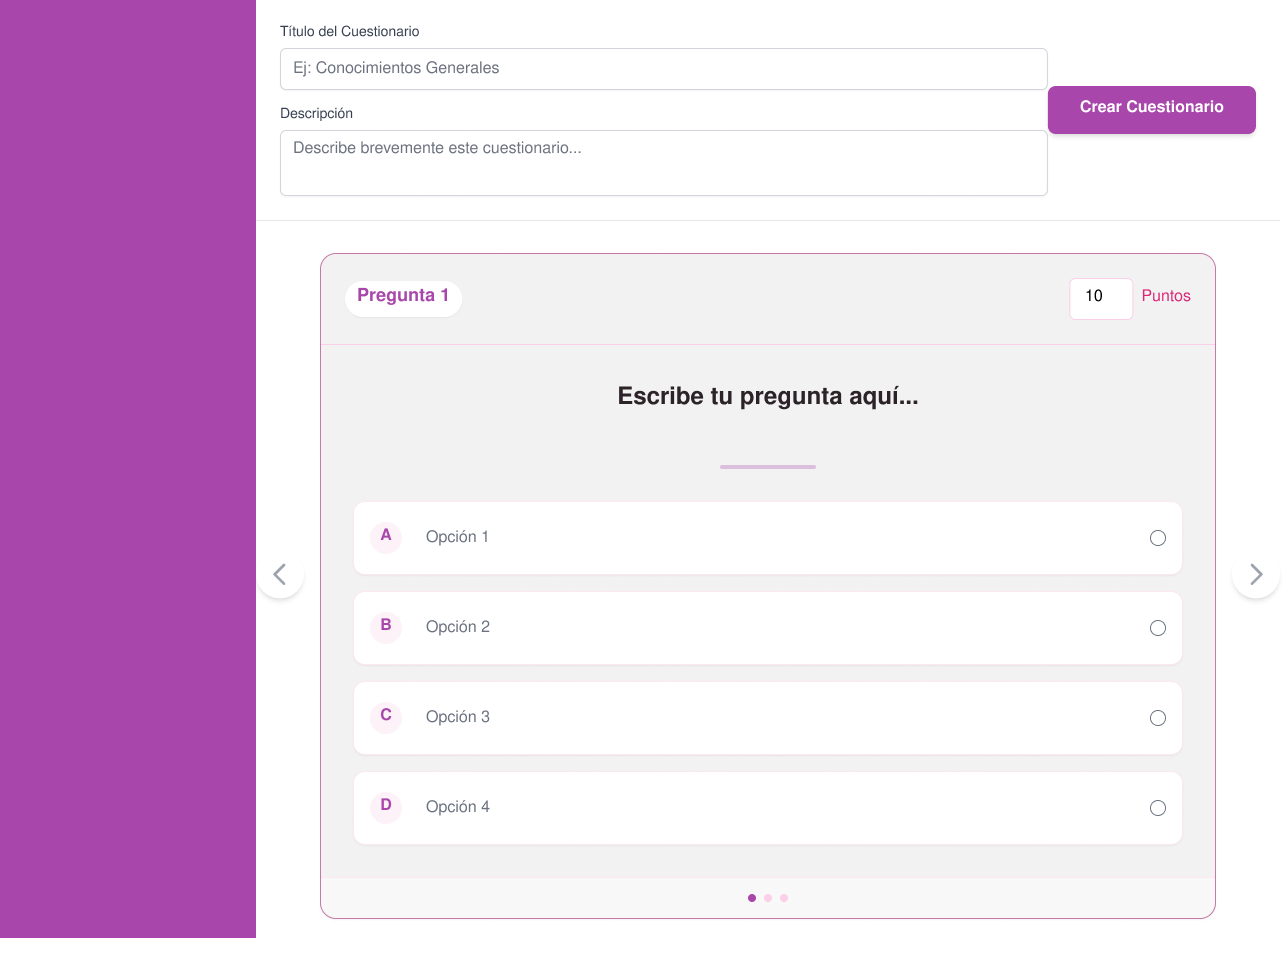
\includegraphics[width=0.75\textwidth]{mockups/02_01_crear_cuestionario.png}
    \caption[Prototipo de creación de cuestionario.]{Crear cuestionario.}
    \label{fig:mockup_crear_cuestionario}
\end{figure}

\begin{figure}[H]
    \centering
    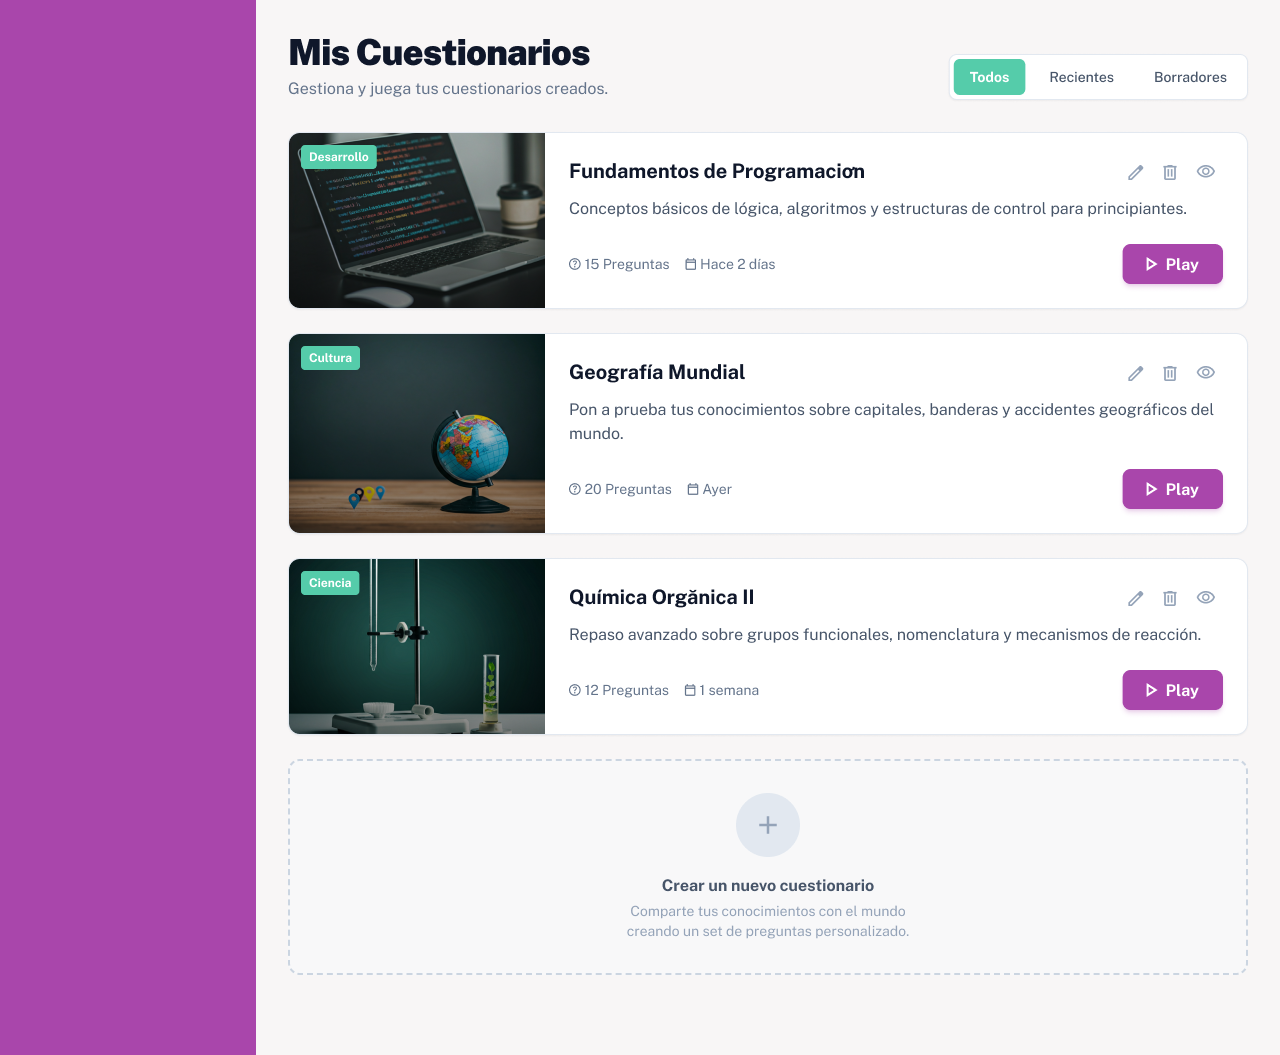
\includegraphics[width=0.7\textwidth]{mockups/02_02_listado_cuestionarios.png}
    \caption[Prototipo de listado de cuestionarios.]{Listado de cuestionarios.}
    \label{fig:mockup_listado_cuestionarios}
\end{figure}

\begin{figure}[H]
    \centering
    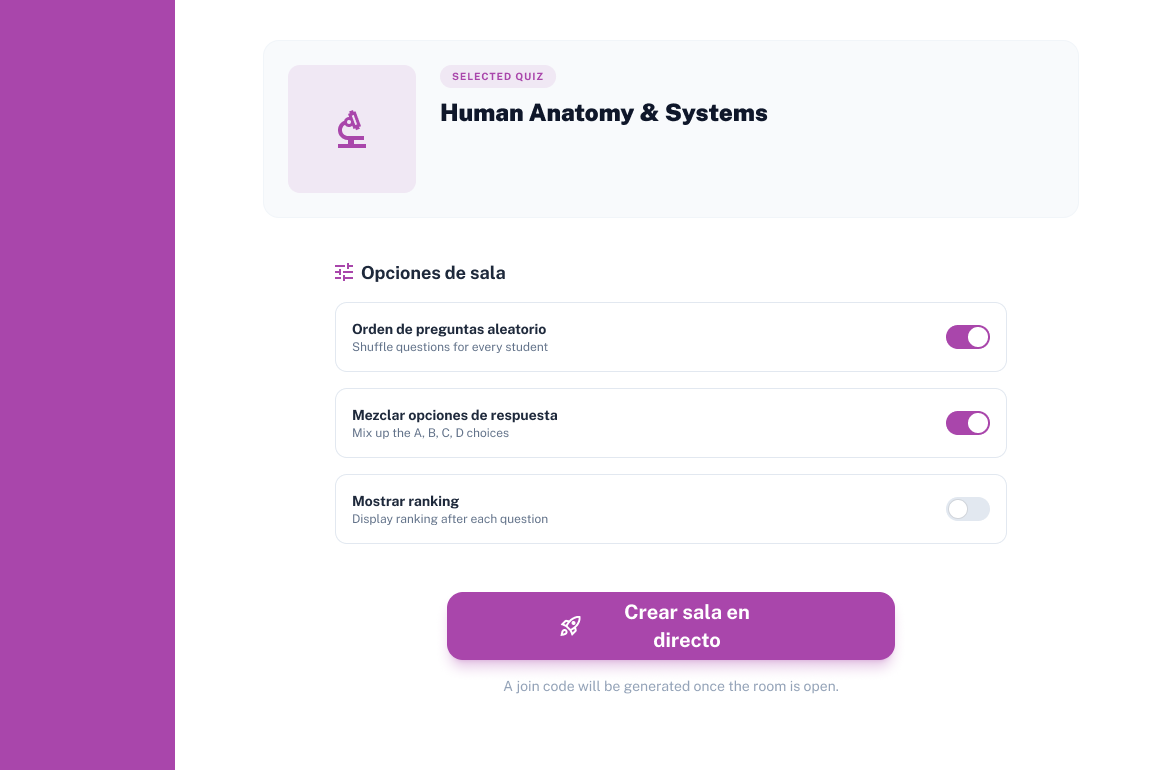
\includegraphics[width=1\textwidth]{mockups/02_03_configuracion_sala.png}
    \caption[Prototipo de configuración de la sala.]{Configuración de la sala.}
    \label{fig:mockup_configuracion_sala}
\end{figure}

\begin{figure}[H]
    \centering
    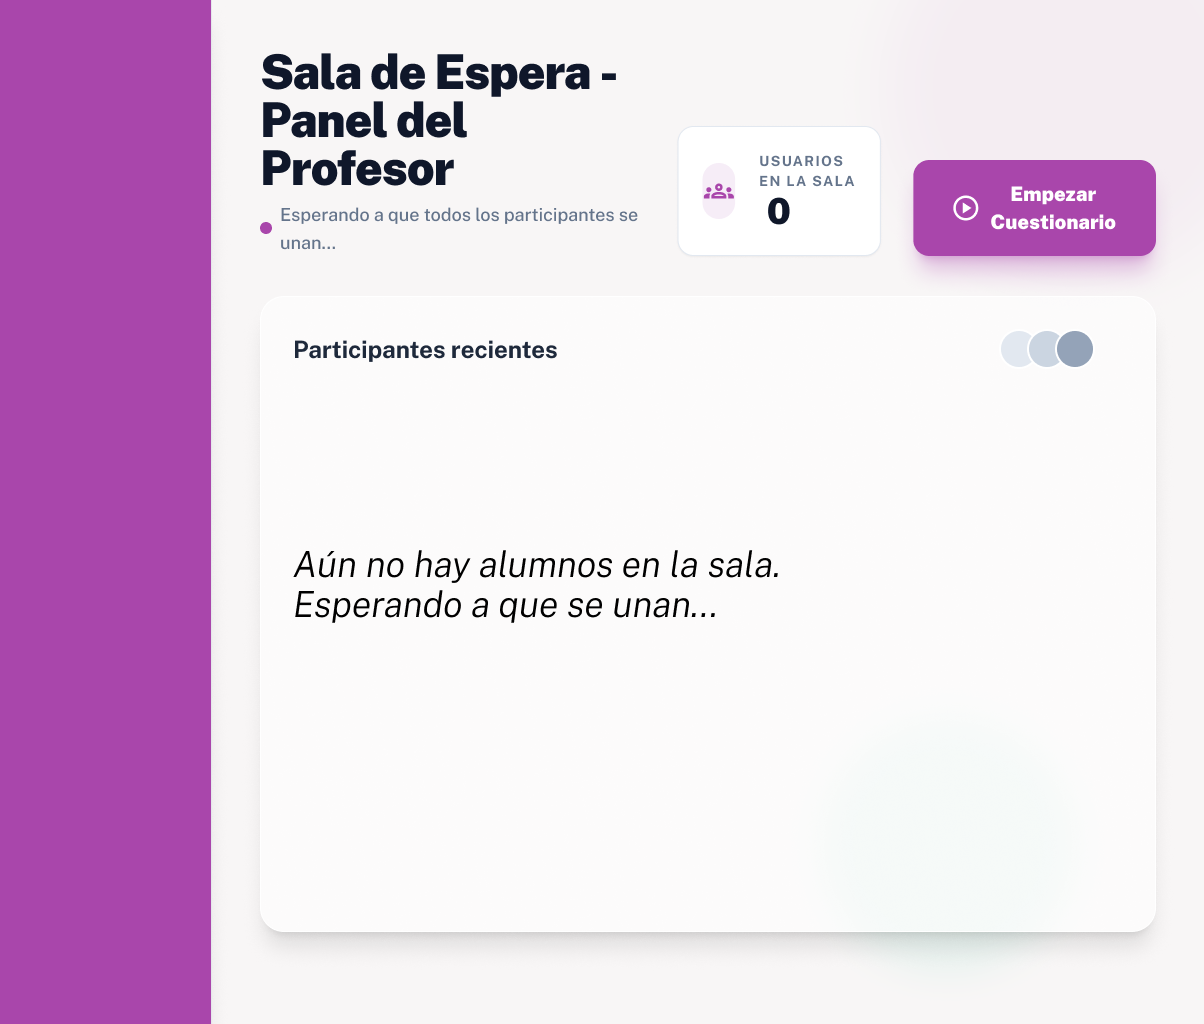
\includegraphics[width=0.8\textwidth]{mockups/02_04_lobby_vacio.png}
    \caption[Prototipo de sala de espera recién creada.]{Sala de espera de la sala recién creada.}
    \label{fig:mockup_lobby_vacio}
\end{figure}

\clearpage

\section*{Flujo de incorporación del estudiante a la sala}
\label{anexo:flujo_incorporacion_estudiante_sala}

Muestra la secuencia que debe seguir un alumno para unirse a una sesión. Inicia con la introducción del código de sala, y continúa con la asignación de su identificador (UVUS o nickname), con su posterior aviso en caso de que el identificador no esté registrado. Por último, muestra la sala de espera hasta el inicio de la partida.

\begin{figure}[H]
    \centering
    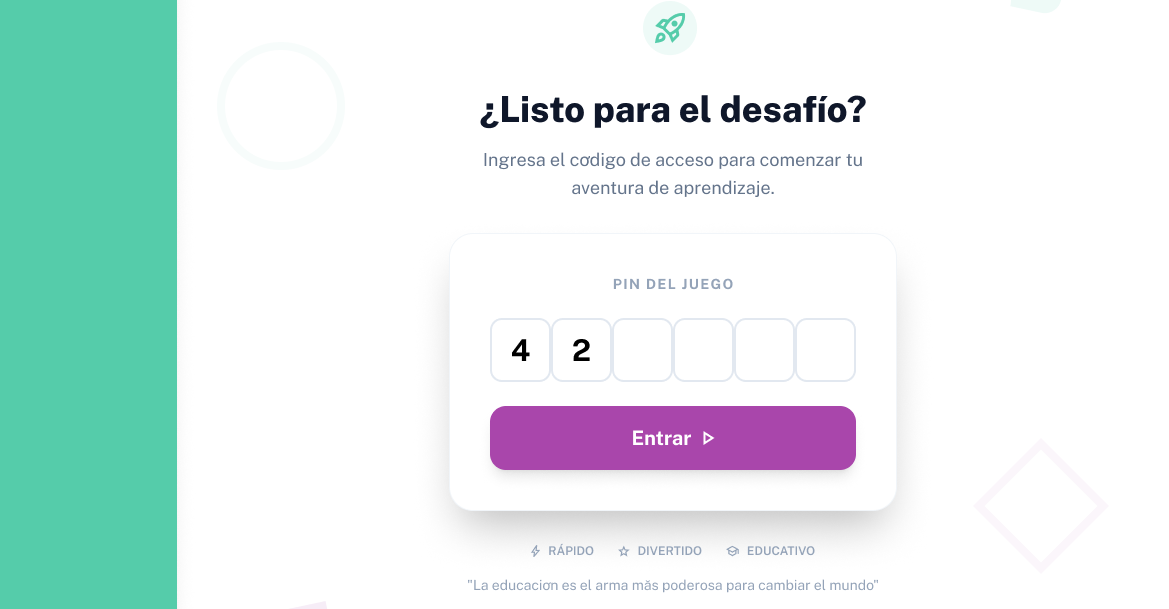
\includegraphics[width=0.95\textwidth]{mockups/03_01_ingresar_codigo.png}
    \caption[Prototipo de \textit{input} de código de sala.]{Ingresar código de sala.}
    \label{fig:mockup_ingresar_codigo}
\end{figure}

\begin{figure}[H]
    \centering
    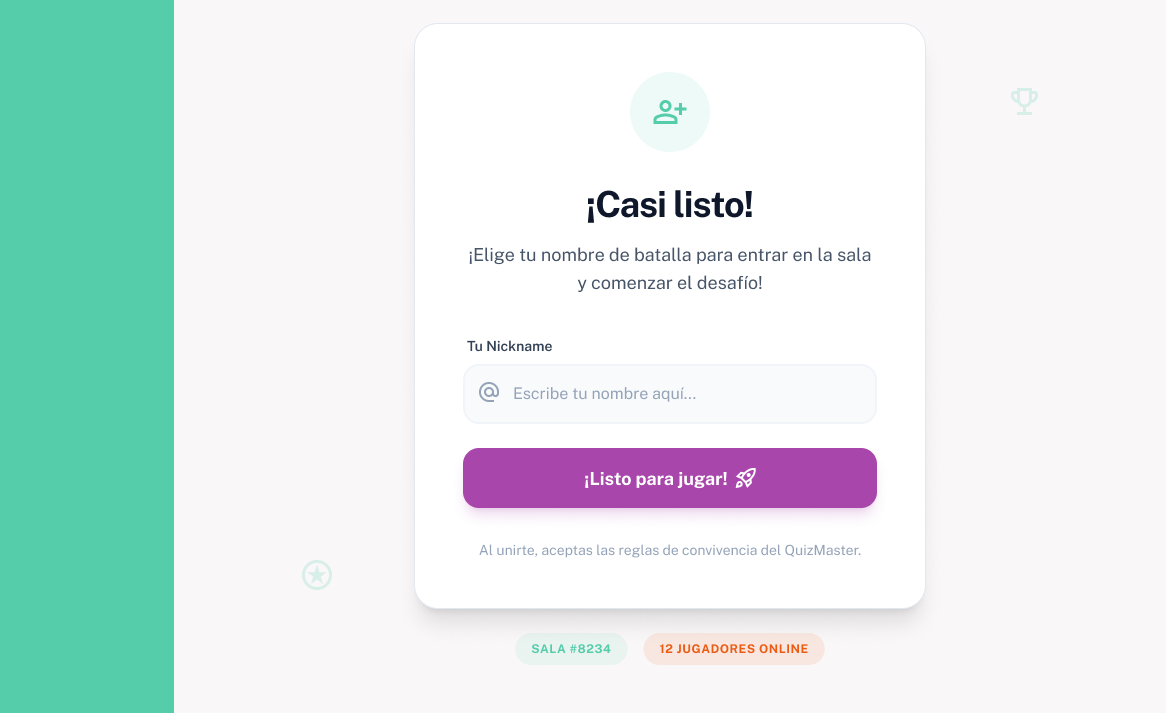
\includegraphics[width=0.95\textwidth]{mockups/03_02_ingresar_nickname.png}
    \caption[Prototipo de \textit{input} de UVUS o nickname.]{Ingresar UVUS o nickname.}
    \label{fig:mockup_ingresar_nickname}
\end{figure}

\begin{figure}[H]
    \centering
    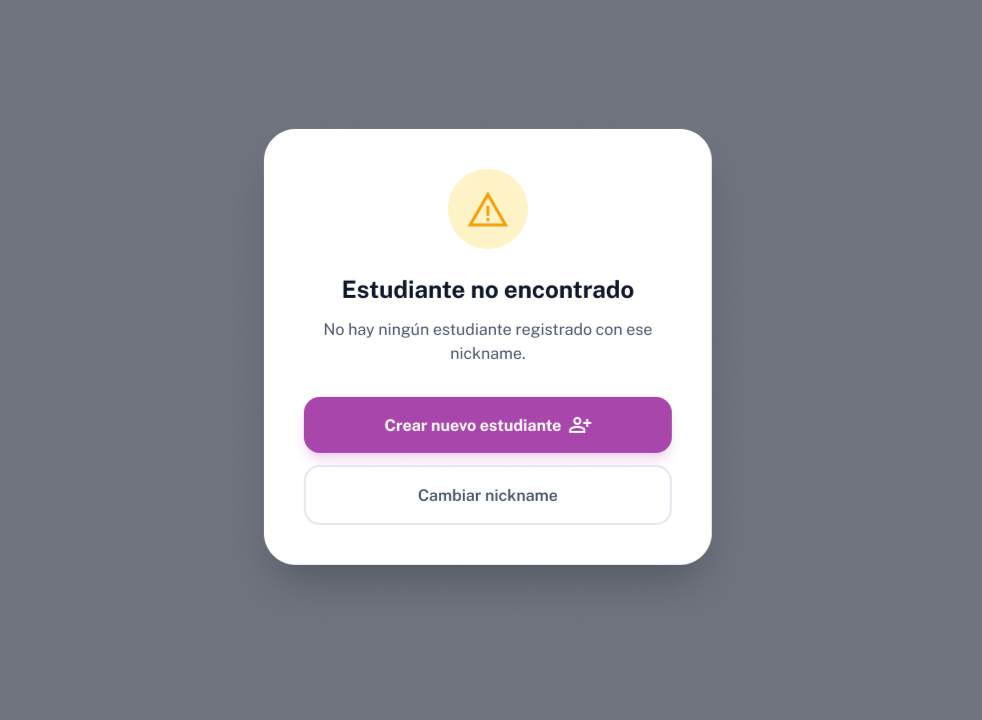
\includegraphics[width=0.9\textwidth]{mockups/03_03_nuevo_nickname.png}
    \caption[Prototipo de aviso para registrar nuevo UVUS o nickname.]{Aviso para registrar nuevo UVUS o nickname.}
    \label{fig:mockup_nuevo_nickname}
\end{figure}

\begin{figure}[H]
    \centering
    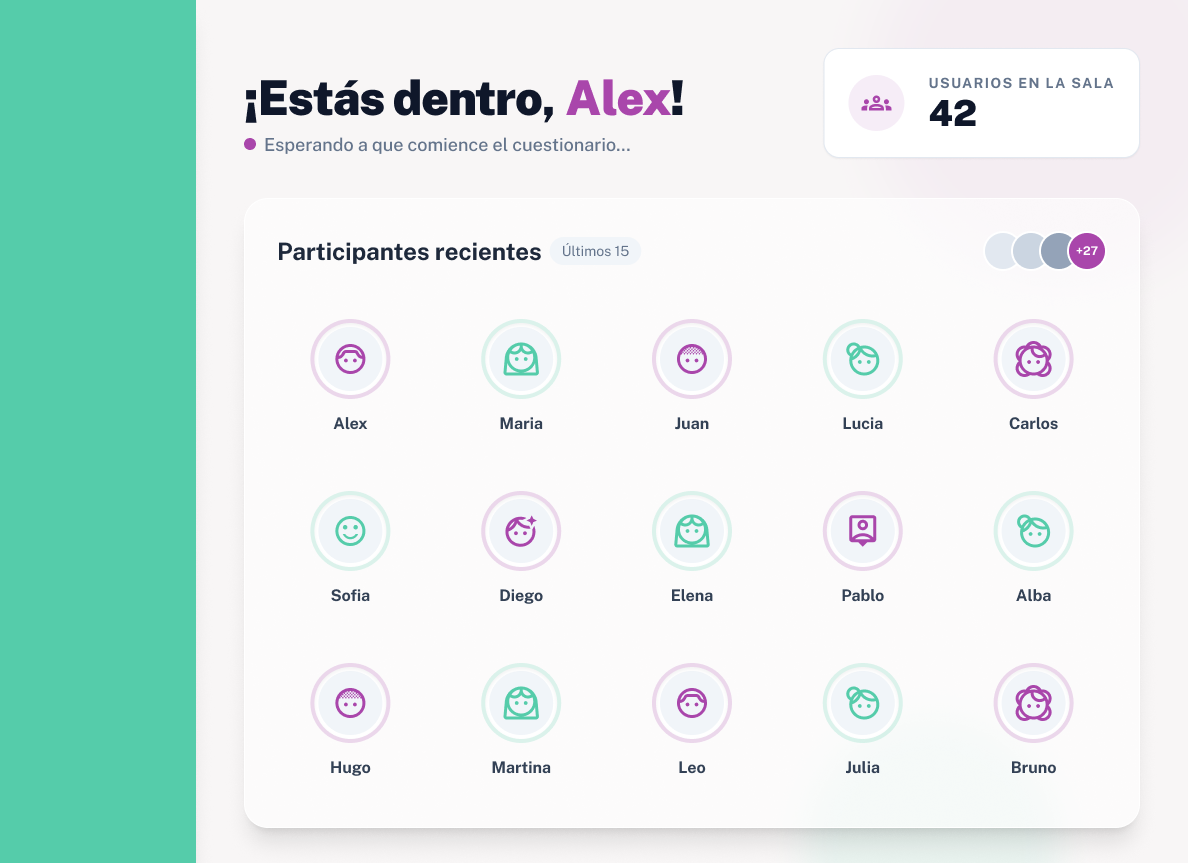
\includegraphics[width=1\textwidth]{mockups/03_04_lobby_alumno.png}
    \caption[Prototipo de sala de espera del alumno recién ingresado.]{Sala de espera del alumno recién ingresado.}
    \label{fig:mockup_lobby_alumno}
\end{figure}

\clearpage

\section*{Flujo de ejecución de la partida en vivo}
\label{anexo:flujo_ejecucion_partida_vivo}

Describe la interacción en tiempo real durante el desarrollo de una sala. Para comparar la experiencia del profesor y del alumno, se presentan en paralelo las interfaces que muestran divergencias funcionales o de diseño. El flujo abarca las fases de sala de espera activa, lectura de pregunta, envío de respuestas, retroalimentación inmediata, tabla de clasificación y verificación final.

\begin{figure}[H]
    \centering
    \makebox[\textwidth][c]{%
        \begin{minipage}{0.57\textwidth}
            \centering
            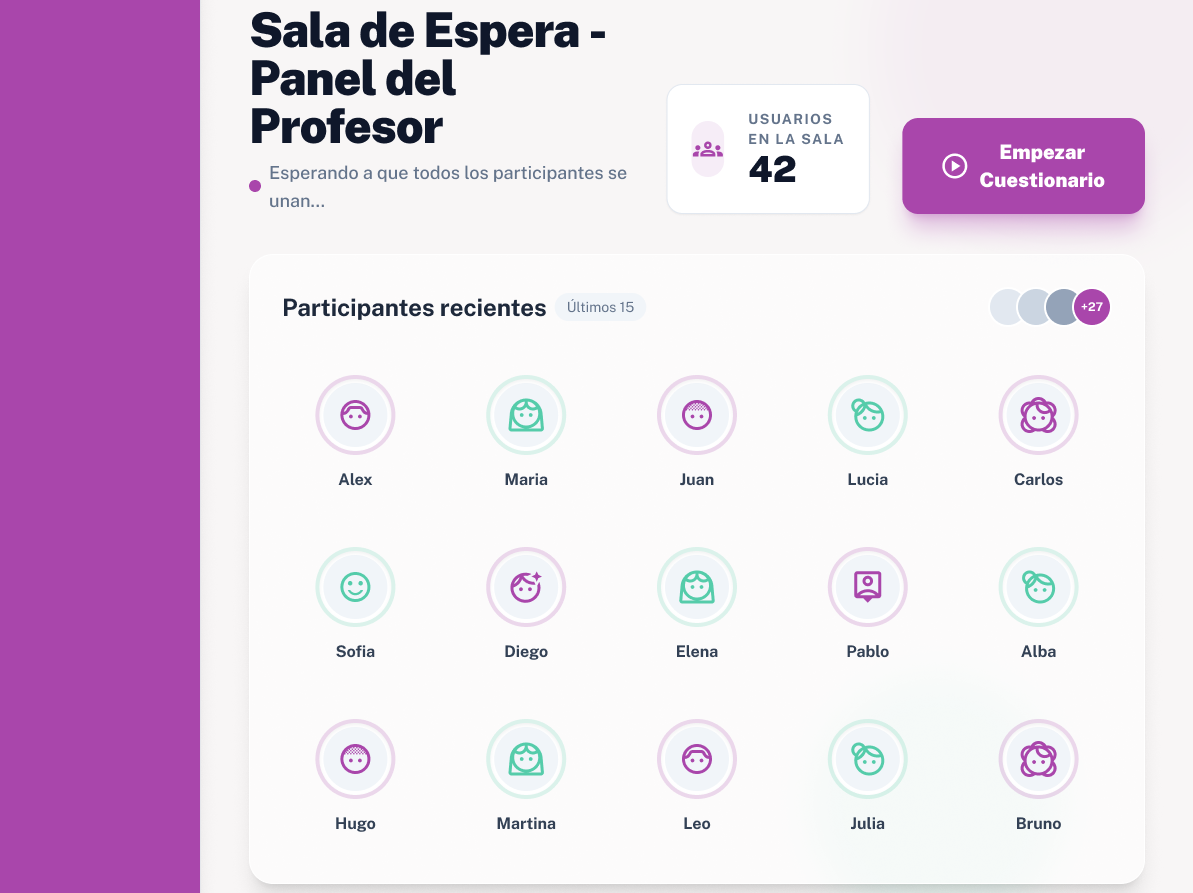
\includegraphics[width=\textwidth]{mockups/04_01_lobby_profesor.png}
            \caption*{Vista Profesor}
        \end{minipage}%
        \hfill
        \begin{minipage}{0.57\textwidth}
            \centering
            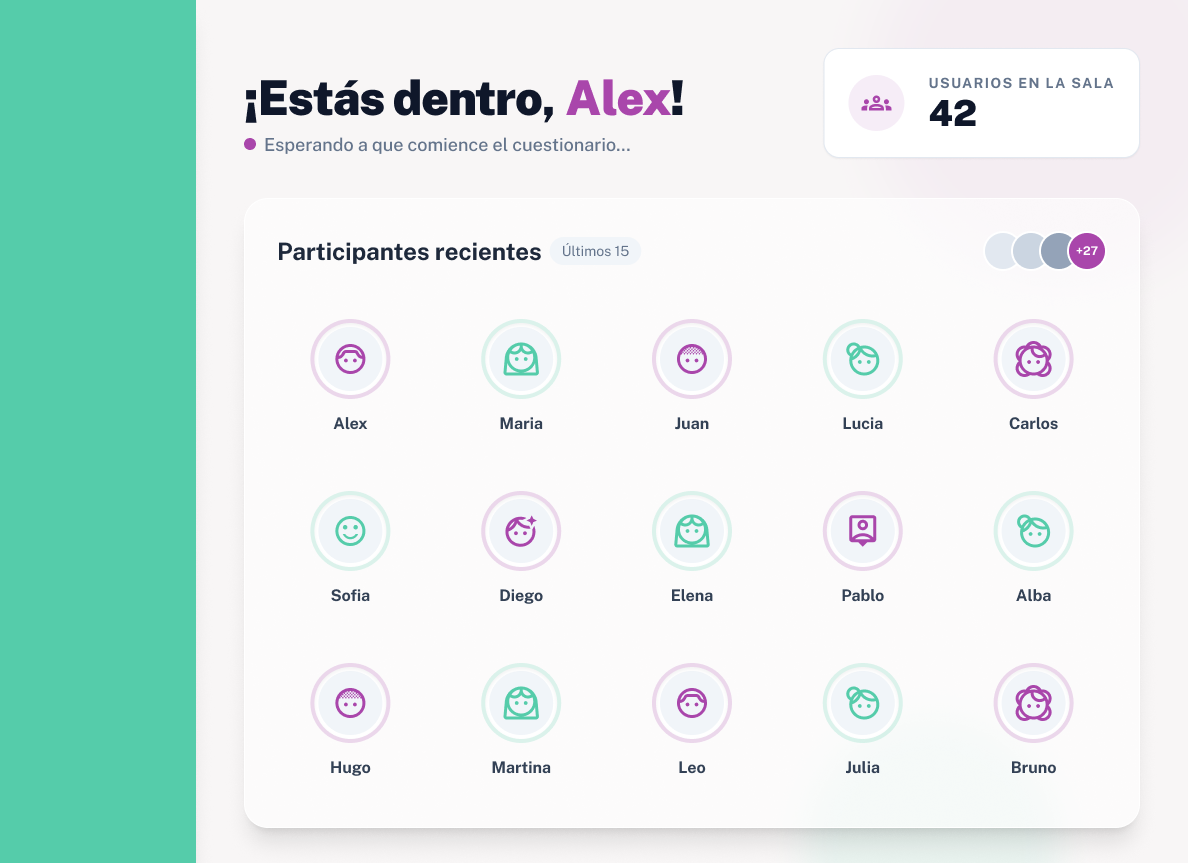
\includegraphics[width=\textwidth]{mockups/04_01_lobby_alumno.png}
            \caption*{Vista Alumno}
        \end{minipage}%
    }
    \caption[Prototipo de sala de espera.]{Sala de espera.}
    \label{fig:mockup_lobby}
\end{figure}

\begin{figure}[H]
    \centering
    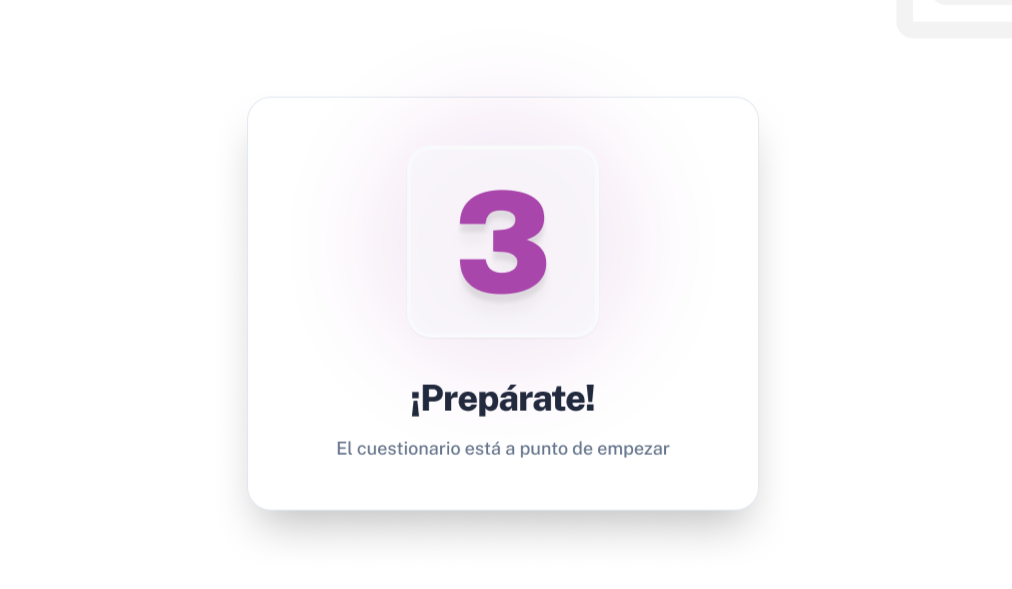
\includegraphics[width=1\textwidth]{mockups/04_02_cuenta_atras.png}
    \caption[Prototipo de cuenta atrás.]{Cuenta atrás.}
    \label{fig:mockup_cuenta_atras}
\end{figure}

\begin{figure}[H]
    \centering
    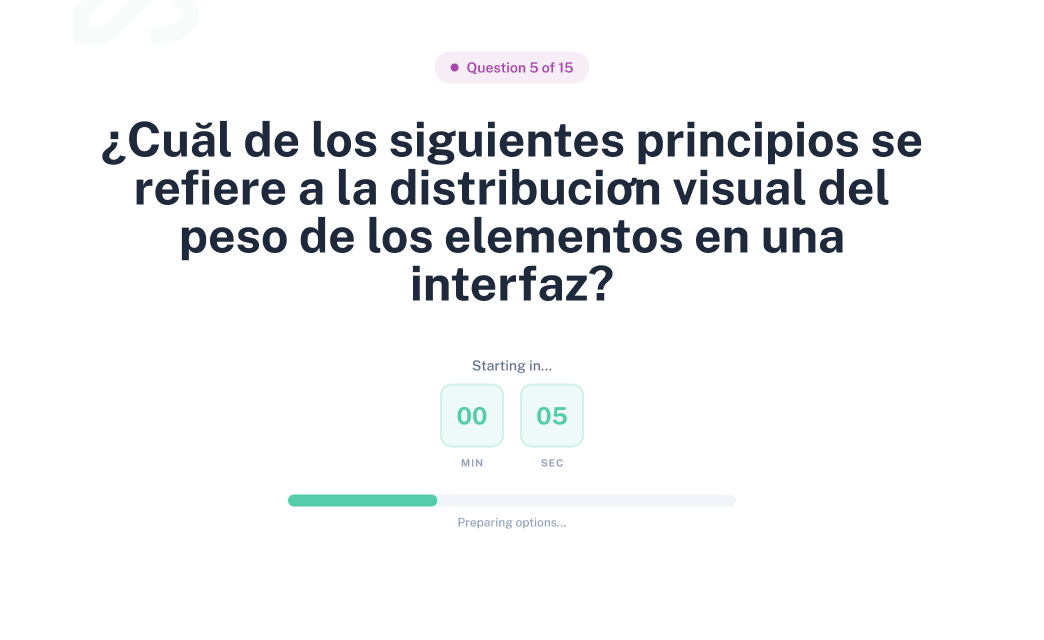
\includegraphics[width=1\textwidth]{mockups/04_03_leer_pregunta.png}
    \caption[Prototipo de tiempo de lectura de pregunta.]{Tiempo de lectura de pregunta.}
    \label{fig:mockup_leer_pregunta}
\end{figure}

\begin{figure}[H]
    \centering
    \makebox[\textwidth][c]{%
        \begin{minipage}{0.57\textwidth}
            \centering
            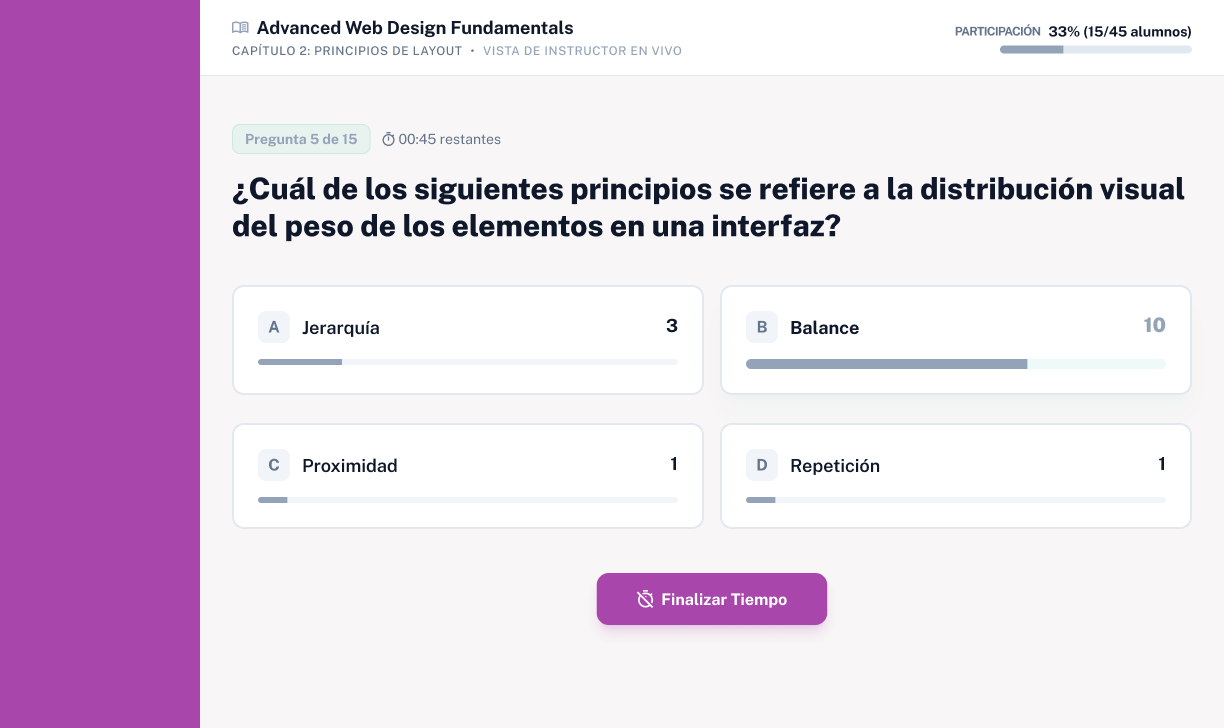
\includegraphics[width=\textwidth]{mockups/04_04_pregunta_profesor.png}
            \caption*{(a) Vista Profesor}
        \end{minipage}%
        \hfill
        \begin{minipage}{0.57\textwidth}
            \centering
            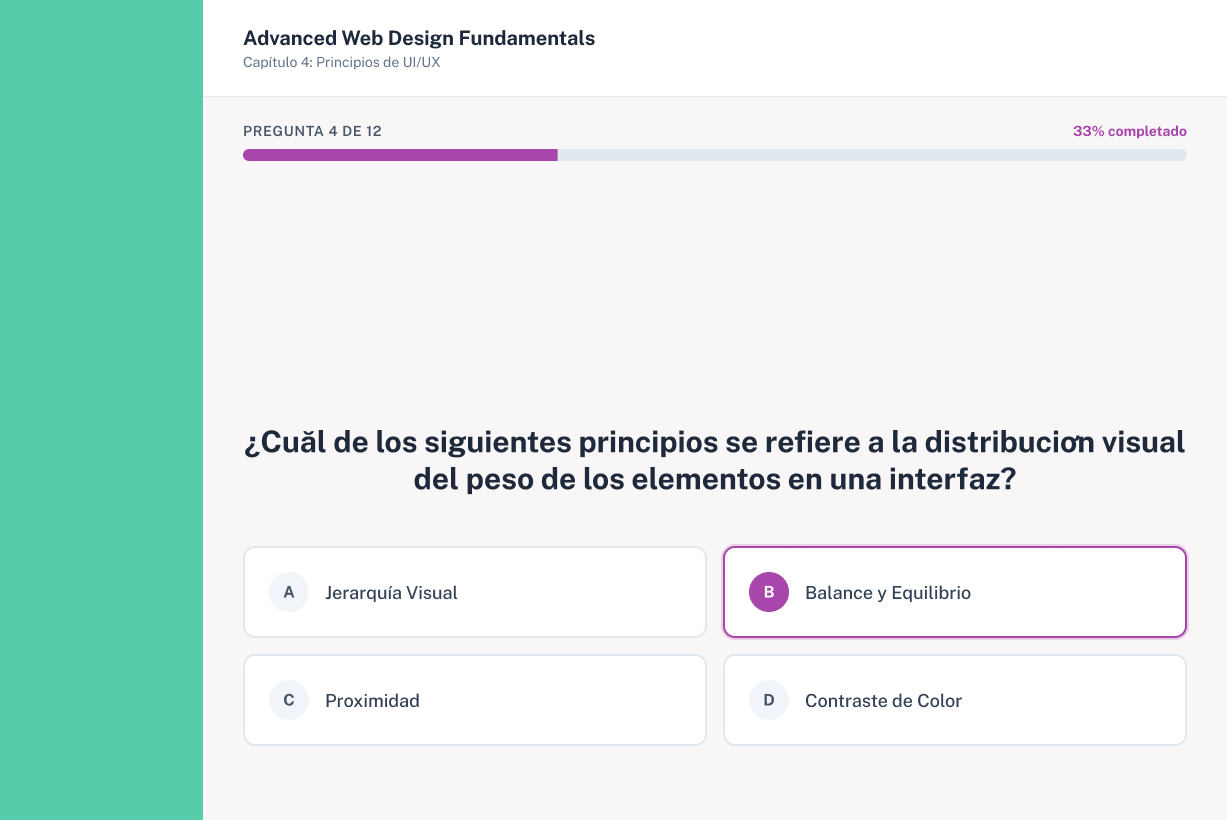
\includegraphics[width=\textwidth]{mockups/04_04_pregunta_alumno.png}
            \caption*{(b) Vista Alumno}
        \end{minipage}%
    }
    \caption[Prototipo de pregunta en curso y envío de respuesta.]{Pregunta en curso y envío de respuesta.}
    \label{fig:mockup_pregunta}
\end{figure}

\begin{figure}[H]
    \centering
    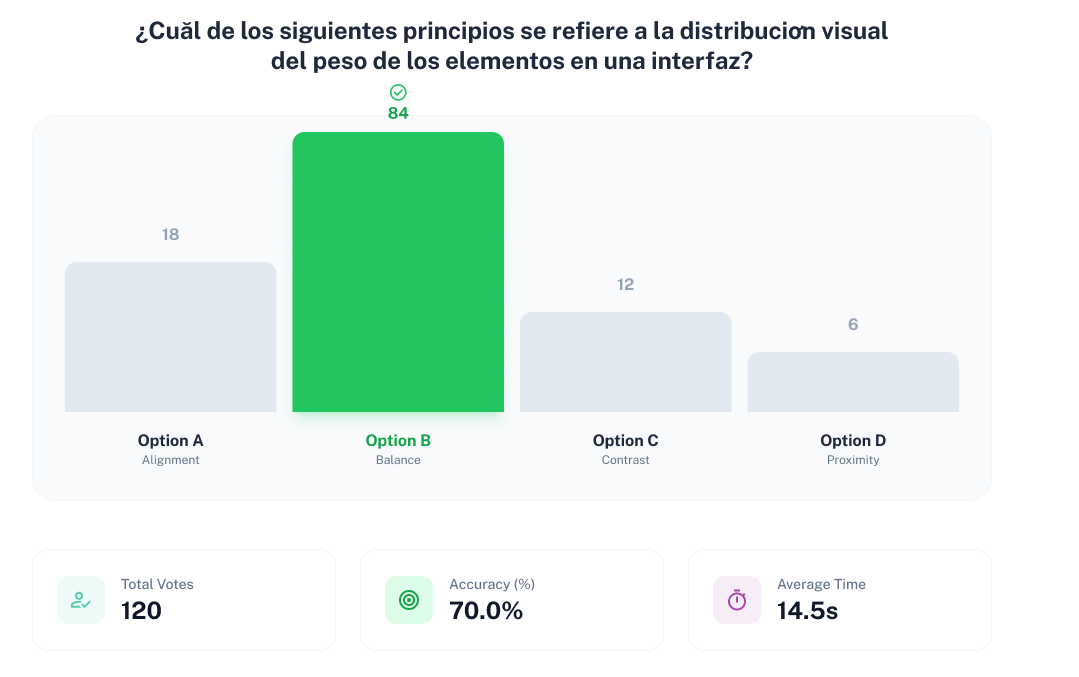
\includegraphics[width=1\textwidth]{mockups/04_05_mostrar_respuesta.png}
    \caption[Prototipo de resultados de la pregunta.]{Resultados de la pregunta.}
    \label{fig:mockup_mostrar_respuesta}
\end{figure}

\begin{figure}[H]
    \centering
    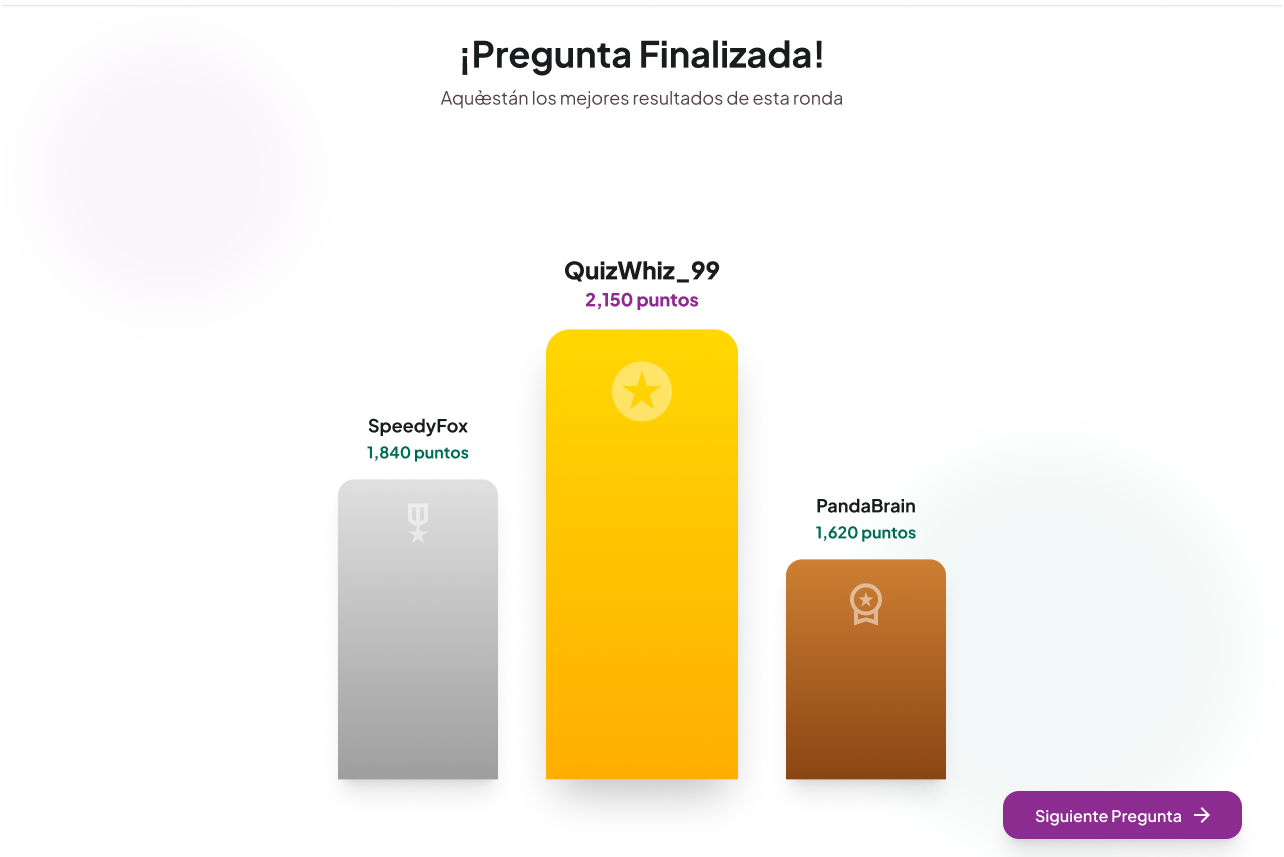
\includegraphics[width=1\textwidth]{mockups/04_06_ranking.png}
    \caption[Prototipo de podio de puntuaciones.]{Podio de puntuaciones.}
    \label{fig:mockup_ranking}
\end{figure}

\begin{figure}[H]
    \centering
    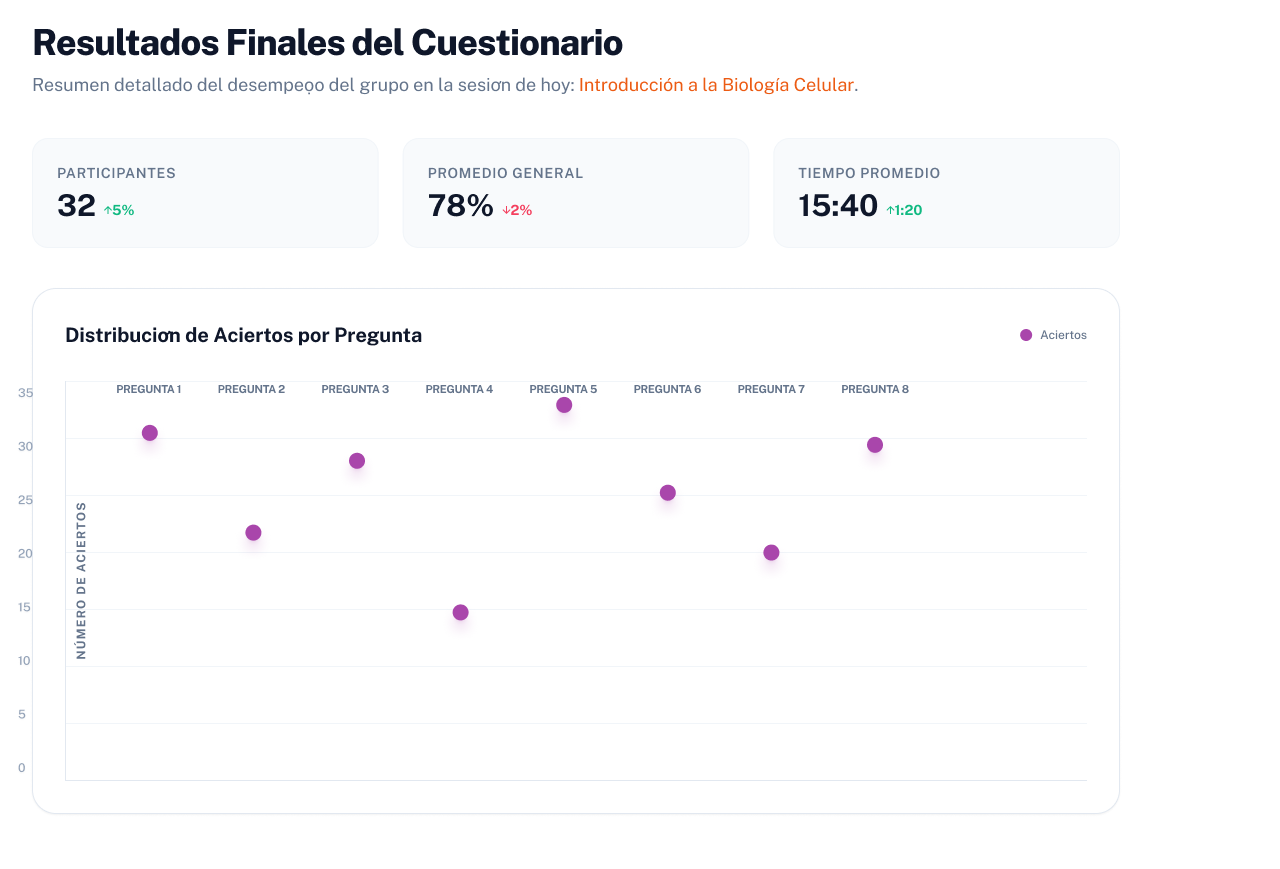
\includegraphics[width=1\textwidth]{mockups/04_07_distribucion_respuestas.png}
    \caption[Prototipo de visualización global de respuestas.]{Distribución global de respuestas.}
    \label{fig:mockup_distribucion_respuestas}
\end{figure}

\begin{figure}[H]
    \centering
    \makebox[\textwidth][c]{%
        \begin{minipage}{0.57\textwidth}
            \centering
            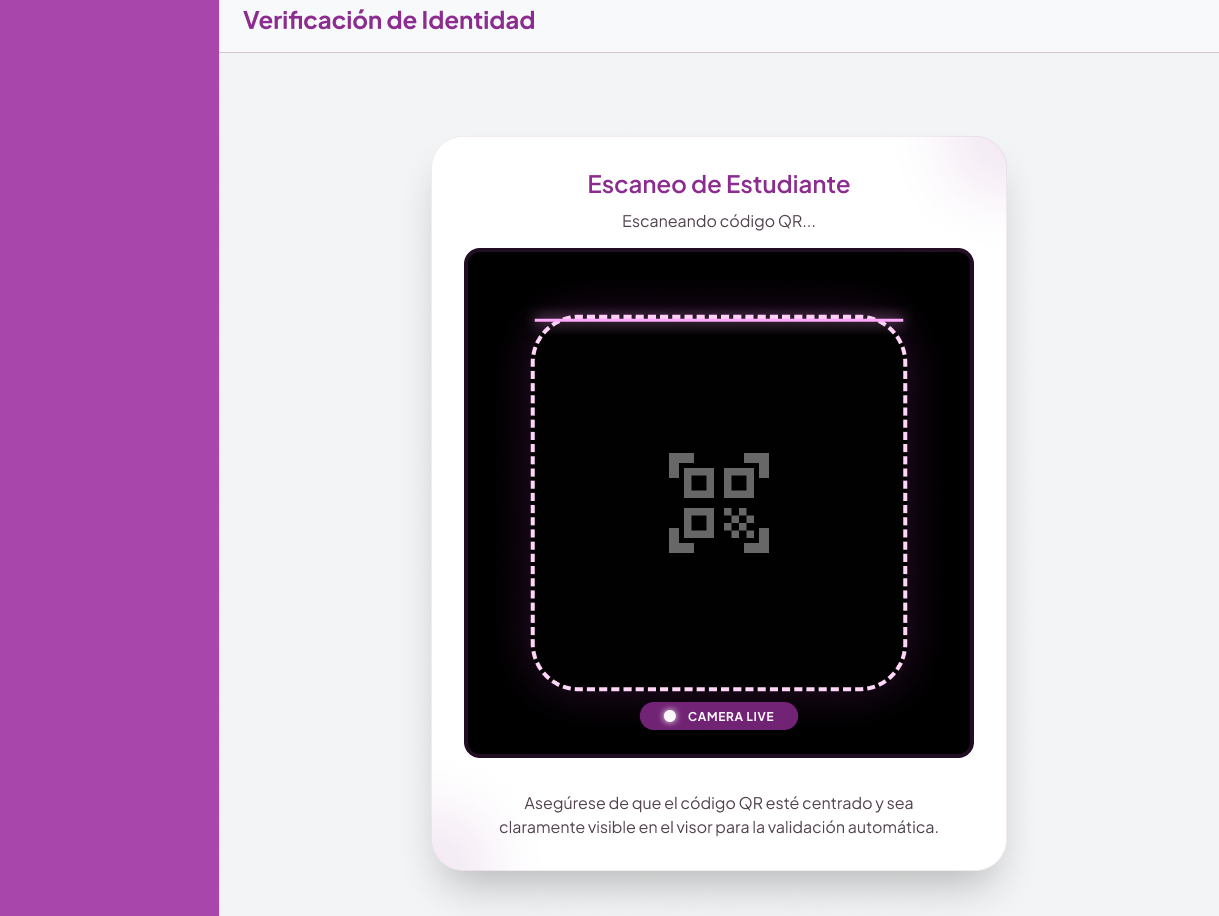
\includegraphics[width=\textwidth]{mockups/04_08_verificacion_profesor.png}
            \caption*{(a) Vista Profesor}
        \end{minipage}%
        \hfill
        \begin{minipage}{0.57\textwidth}
            \centering
            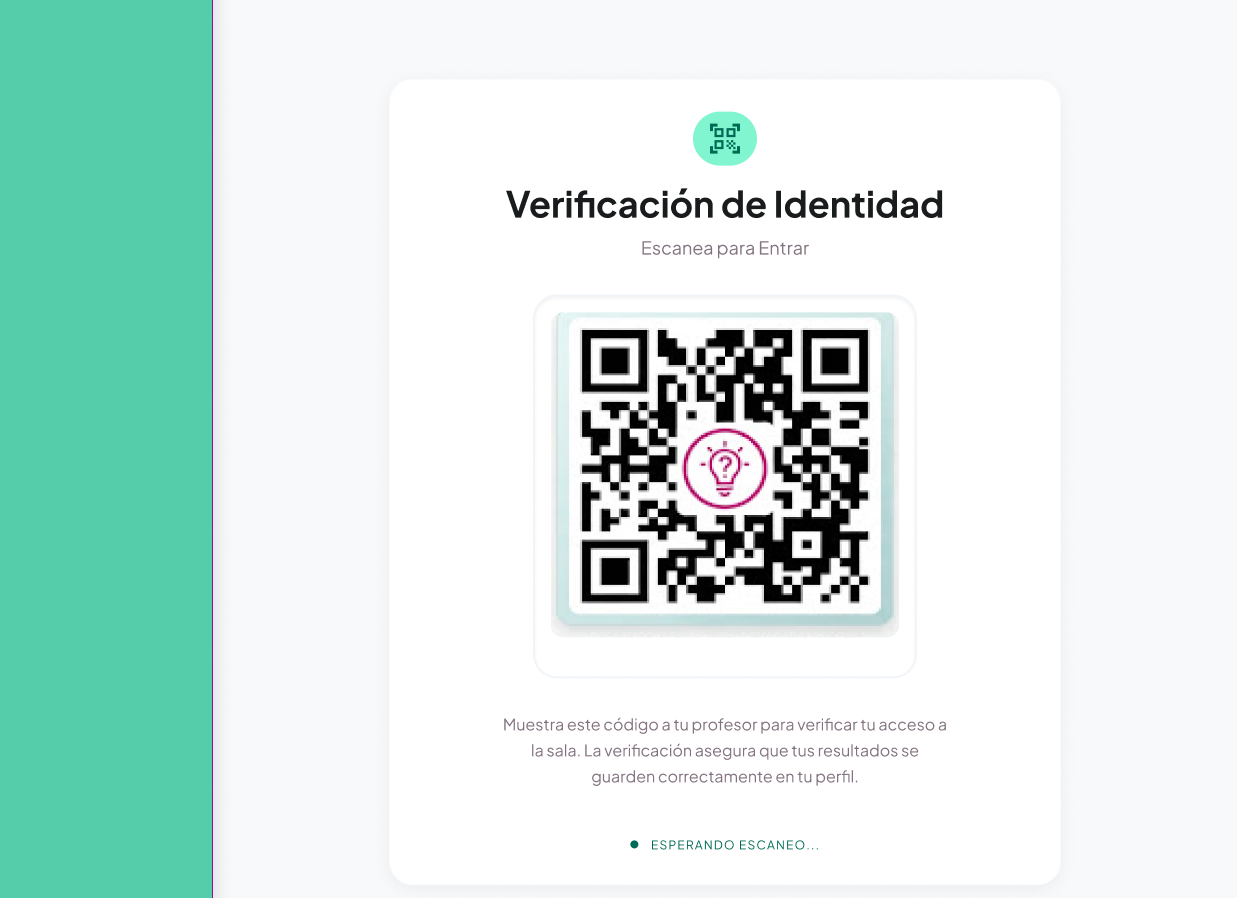
\includegraphics[width=\textwidth]{mockups/04_08_verificacion_alumno.png}
            \caption*{(b) Vista Alumno}
        \end{minipage}%
    }
    \caption[Prototipo de verificación final.]{Verificación final.}
    \label{fig:mockup_verificacion}
\end{figure}

\end{appendices}